\subsection{Structure}
\begin{definition}
    Each vertex in a decision tree is either:
    \begin{enumerate}
        \item A \textbf{condition vertex}: a vertex that sorts points based on a question.
        \item A \textbf{decision vertex}: a vertex that assigns all points a specific class.
    \end{enumerate}
\end{definition}

\begin{notes}
    We want to find the minimum \# of condition vertices (or questions) needed to "sufficiently discriminate" (identify the class of every point in \(\mathcal{D}\)).
    \begin{itemize}
        \item More condition vertices improve discrimination.
        \item Less condition vertices improve generalization.
    \end{itemize}
\end{notes}

\subsection{Building a Decision Tree}
\begin{definition}
    Consider determining the calss of a randomly chosen target point. 
    \begin{itemize}
        \item If we ask a $K$-ary question abt. the pts. in $\mathcal{D}$, we can form $K$ subsets, $\mathcal{D}^{(1)},\ldots,\mathcal{D}^{(K)}$, using the answers s.t. 
        \begin{itemize}
            \item $|\mathcal{D}^{(k)}| \in \{0,\ldots,|\mathcal{D}|\}$
            \item $|\mathcal{D}| = \sum_{k=1}^{K} |\mathcal{D}^{(k)}|$
        \end{itemize}
    \end{itemize}
\end{definition}

\subsubsection{Special Case}
\begin{notes}
    Suppose each pt. belongs to a unique class (i.e. the \# of classes is $|\mathcal{D}|$).
    \customFigure[0.5]{../Images/L5_10.png}{}
    \begin{enumerate}
    \item Before asking the question: \( |\mathcal{D}| \) possible guesses for the target point’s class.
    \item After asking the question: Either 
    \begin{itemize}
        \item \( |\mathcal{D}^{(1)}|, \dots, |\mathcal{D}^{(K-1)}| \) or 
        \item \( |\mathcal{D}^{(K)}| \) 
    \end{itemize}
    guesses, depending on the answer for the target point.

    \item Goal: Minimize the \# of guesses needed in the worst-case, which would be 
    \[
    \max \{ |\mathcal{D}^{(1)}|, \dots, |\mathcal{D}^{(K)}| \}.
    \]

    \item Given the constraints on \( |\mathcal{D}^{(1)}|, \dots, |\mathcal{D}^{(K)}| \), we can show that $\max \{ |\mathcal{D}^{(1)}|, \dots, |\mathcal{D}^{(K)}| \}$ is minimized when
    \[
    |\mathcal{D}^{(K)}| \in \left\{ \left\lfloor \frac{|\mathcal{D}|}{K} \right\rfloor, \left\lceil \frac{|\mathcal{D}|}{K} \right\rceil \right\}.
    \]

    Basically, the best question splits \( \mathcal{D} \) into \( K \) sets of (roughly) the same size.
    \end{enumerate}
\end{notes}

\begin{warning}
    Roughly due to floor/ceil.
\end{warning}

\begin{theorem}
    Given a classification data-set, \( \mathcal{D} \), in which the class of each point is unique (i.e., \( |\text{out}(\mathcal{D})| = |\mathcal{D}| \)), the class of a randomly chosen target point can be determined within 
    \[
    \lceil \log_K (|\mathcal{D}|) \rceil
    \]
    \( K \)-ary questions.

\end{theorem}

\subsubsection{General Case}
\begin{motivation}
    Suppose points do not necessarily belong to a unique class.
    \vspace{1em}

    In the context of decision trees:
    \begin{itemize}
        \item \(X\) is the class of a randomly chosen target point.
        \item \(Y\) is the answer to a \(K\)-ary question for \(X\).
    \end{itemize}

    Maximize \(IG(X|Y)\) (i.e. choose the question to maximize the information gained).
\end{motivation}

\subsubsection{Entropy, Conditional Entropy, and Information Gain}
\begin{definition}
    The \textbf{entropy} of a random variable \(X\) (in \(K\)-its) is defined as
    \begin{equation*}
        H(X) = -\sum_{\forall x \in X} p_X(x) \log_K(p_X(x)).
    \end{equation*}

    The \textbf{conditional entropy} of a random variable, \(X\), given a random variable \(Y\), is
    \begin{equation*}
        H(X|Y) = -\sum_{\forall y \in Y} \sum_{\forall x \in X} p_{X|Y}(x | y) \log_K(p_{X|Y}(x|y)).
    \end{equation*}

    The \textbf{information gain} from \(Y\) is:
    \begin{equation*}
        IG(X|Y) = H(X) - H(X|Y).
    \end{equation*}
\end{definition}

\begin{warning}
    \begin{itemize}
        \item There are $\infty$ many potential questions, but there are only finite many ways to split the dataset. 
    \end{itemize}
\end{warning}
\newpage

\begin{process}
    \begin{enumerate}
        \item Calculate \(H(X)\) (i.e. entropy before the split).
        \item Calculate \(H(X|Y)\) (i.e. entropy after the split).
        \begin{enumerate}
            \item Calculate entropy for each subset of \(X\) based on the question, \(Y\).
            \item Calculate the weighted average of the entropies.
        \end{enumerate}
        \item Calculate \(IG(X|Y) = H(X) - H(X|Y)\).
    \end{enumerate}
\end{process}

\begin{example}
    \customFigure[0.5]{../Images/L5_0.png}{}    
\end{example}
\newpage

\begin{example} \textbf{2-Ary Question}
    \begin{enumerate}
        \item \textbf{Given:} $X= \{0,1,2\}$, $Y = 
        \begin{cases} 
        1, & \text{if } x_1 \leq 3 \quad (\text{Yes}) \\
        0, & \text{if } x_1 > 3 \quad (\text{No})
        \end{cases}$, 
        \item \textbf{Problem:} $IG(X|Y) = ?$
        \item \textbf{Solution:}
        \begin{enumerate}
            \item Entropy before the split: $H(X) = \frac{3}{10} \log_2\left(\frac{10}{3}\right) + \frac{2}{10} \log_2\left(\frac{10}{2}\right) + \frac{5}{10} \log_2\left(\frac{10}{5}\right)$
            \item Entropy after the split: 
            \begin{enumerate}
                \item $H(X \mid x_1 \leq 3) = \frac{3}{5} \log_2 \left(\frac{5}{3}\right) + \frac{2}{5} \log_2 \left(\frac{5}{2}\right)$ 
                \item $H(X \mid x_1 > 3) = \frac{2}{5} \log_2 \left(\frac{5}{2}\right) + \frac{3}{5} \log_2 \left(\frac{5}{3}\right)$.
                \item Weighted Avg. Entropy: $H(X|Y) = \frac{5}{10} H(X \mid x_1 \leq 3) + \frac{5}{10} H(X \mid x_1 > 3)$
            \end{enumerate}
            \item $IG(X|Y) = H(X) - H(X|Y)$
        \end{enumerate}
    \end{enumerate}
\end{example}

\begin{example} \textbf{2-Ary Question}
    \begin{enumerate}
        \item \textbf{Given:} $X= \{0,1,2\}$, $Y = 
        \begin{cases} 
        1, & \text{if } x_2 \leq 3 \quad (\text{Yes}) \\
        0, & \text{if } x_2 > 3 \quad (\text{No})
        \end{cases}$, 
        \item \textbf{Problem:} $IG(X|Y) = ?$
        \item \textbf{Solution:}
        \begin{enumerate}
            \item Entropy before the split: $H(X) = \frac{3}{10} \log_2\left(\frac{10}{3}\right) + \frac{2}{10} \log_2\left(\frac{10}{2}\right) + \frac{5}{10} \log_2\left(\frac{10}{5}\right)$
            \item Entropy after the split: 
            \begin{enumerate}
                \item $H(X \mid x_2 > 3) = \frac{3}{3} \log_2 \left(\frac{3}{3}\right)$ 
                \item $H(X \mid x_2 \leq 3) = \frac{3}{5} \log_2 \left(\frac{5}{3}\right) + \frac{2}{5} \log_2 \left(\frac{5}{2}\right)+ \frac{2}{5} \log_2 \left(\frac{5}{2}\right)$.
                \item Weighted Avg. Entropy: $H(X|Y) = \frac{3}{10} H(X \mid x_2 > 3) + \frac{7}{10} H(X \mid x_2 \leq 3)$
            \end{enumerate}
            \item $IG(X|Y) = H(X) - H(X|Y)$
        \end{enumerate}
    \end{enumerate}
\end{example}

\begin{example} \textbf{3-Ary Question}
    \begin{enumerate}
        \item \textbf{Given:} $X= \{0,1,2\}$, $Y = \begin{cases}
        1, & \text{if } x_1 \leq 3 \text{ and } x_2 \leq 3 \\
        2, & \text{if } x_1 \leq 3 \text{ and } x_2 > 3 \\
        3, & \text{if } x_1 > 3 
        \end{cases}$
        \item \textbf{Problem:} $IG(X|Y) = ?$
        \item \textbf{Solution:}
        \begin{enumerate}
            \item Entropy before the split: $H(X) = \frac{3}{10} \log_2\left(\frac{10}{3}\right) + \frac{2}{10} \log_2\left(\frac{10}{2}\right) + \frac{5}{10} \log_2\left(\frac{10}{5}\right)$
            \item Entropy after the split:
            \begin{enumerate}
                \item $H(X \mid x_1 \leq 3 \text{ and } x_2 \leq 3) = \frac{3}{3} \log_2\left(\frac{3}{3}\right)$
                \item $H(X \mid x_1 \leq 3 \text{ and } x_2 > 3) = \frac{2}{2} \log_2\left(\frac{2}{2}\right)$
                \item $H(X \mid x_1 > 3) = \frac{2}{5} \log_2\left(\frac{5}{2}\right) + \frac{3}{5} \log_2\left(\frac{5}{3}\right)$
                \item $H(X|Y) = \frac{3}{10} H(X \mid x_1 \leq 3 \text{ and } x_2 \leq 3) + \frac{2}{10} H(X \mid x_1 \leq 3 \text{ and } x_2 > 3) + \frac{5}{10} H(X \mid x_1 > 3)$
            \end{enumerate}
            \item $IG(X|Y) = H(X) - H(X|Y)$
        \end{enumerate}
    \end{enumerate}
\end{example}
\newpage

\begin{example} \textbf{Decision Tree}
    \begin{enumerate}
        \item \textbf{Given:} $X= \{0,1,2\}$
        \item \textbf{Problem:} Draw a decision tree using binary conditions of the form, \(x_i \leq k\), where \(i \in \{1, 2\}\) and \(k \in \mathbb{Z}\), that maximizes the information gained at each level.
        \item \textbf{Solution (Level 1):}
        \begin{enumerate}
            \item Entropy before the split: $H(X) = \frac{3}{10} \log_2\left(\frac{10}{3}\right) + \frac{2}{10} \log_2\left(\frac{10}{2}\right) + \frac{5}{10} \log_2\left(\frac{10}{5}\right) = 1.485 [\text{bits}]$
            \item Entropy after the split and information gain (everything in base 2 since 2-ary).
        \end{enumerate}
    \end{enumerate}
    \begin{center}
        \begin{tabular}{ll}
            \textbf{Split} & \textbf{Entropy} \\
            \toprule
            \(x_1 \leq 1\) & $H(X | Y) = \frac{3}{10} \left[\frac{2}{3} \log \left(\frac{3}{2}\right) + \frac{1}{3} \log \left(\frac{3}{1}\right) \right] + \frac{7}{10} \left[\frac{1}{7} \log \left(\frac{7}{1}\right) + \frac{2}{7} \log \left(\frac{7}{2}\right) + \frac{4}{7} \log \left(\frac{7}{4}\right) \right] = 1.241 [\text{bits}]$ \\
            \multicolumn{2}{p{\linewidth}}{
            \begin{itemize}
                \item $IG(X|Y) = 1.485 - 1.241 = 0.244 [\text{bits}]$
            \end{itemize}} \\
            \midrule
            $x_1 \leq 2,3$ & $H(X | Y) = \frac{5}{10} \left[\frac{3}{5} \log \left(\frac{5}{3}\right) + \frac{2}{5} \log \left(\frac{5}{2}\right) \right] + \frac{5}{10} \left[\frac{2}{5} \log \left(\frac{5}{2}\right) + \frac{3}{5} \log \left(\frac{5}{3}\right) \right] = 0.971 [\text{bits}]$ \\
            \multicolumn{2}{p{\linewidth}}{
            \begin{itemize}
                \item $\boxed{IG(X|Y) = 1.485 - 0.971 = 0.514 [\text{bits}]}$
            \end{itemize}} \\
            \midrule
            $x_1 \leq 4,5$ & $H(X | Y) = \frac{8}{10} \left[\frac{3}{8} \log \left(\frac{8}{3}\right) + \frac{2}{8} \log \left(\frac{8}{2}\right) + \frac{3}{8} \log \left(\frac{8}{3}\right) \right] + \frac{2}{10} \left[\frac{2}{2} \log \left(\frac{2}{2}\right) \right] = 1.249 [\text{bits}]$ \\
            \multicolumn{2}{p{\linewidth}}{
            \begin{itemize}
                \item $IG(X|Y) = 1.485 - 1.249 = 0.236 [\text{bits}]$
            \end{itemize}} \\
            \midrule
            $x_1 \leq 6$ & $H(X | Y) = \frac{10}{10} \left[\frac{3}{10} \log \left(\frac{10}{3}\right) + \frac{2}{10} \log \left(\frac{10}{2}\right) + \frac{5}{10} \log \left(\frac{10}{5}\right) \right] = 1.485 [\text{bits}]$ \\
            \multicolumn{2}{p{\linewidth}}{
            \begin{itemize}
                \item $IG(X|Y) = 1.485 - 1.485 = 0 [\text{bits}]$
            \end{itemize}} \\
            \midrule 
            $x_2 \leq 1$ & $H(X | Y) = \frac{4}{10} \left[\frac{2}{4} \log \left(\frac{4}{2}\right) + \frac{1}{4} \log \left(\frac{4}{1}\right) + \frac{1}{4} \log \left(\frac{4}{1}\right) \right] + \frac{6}{10} \left[2 \cdot \frac{1}{6} \log \left(\frac{6}{1}\right) + \frac{4}{6} \log \left(\frac{6}{4}\right) \right] = 1.351 [\text{bits}]$ \\
            \multicolumn{2}{p{\linewidth}}{
            \begin{itemize}
                \item $IG(X|Y) = 1.485 - 1.351 = 0.134 [\text{bits}]$
            \end{itemize}} \\
            \midrule 
            $x_2 \leq 2,3$ & $H(X | Y) = \frac{7}{10} \left[\frac{3}{7} \log \left(\frac{7}{3}\right) + \frac{2}{7} \log \left(\frac{7}{2}\right) + \frac{2}{7} \log \left(\frac{7}{2}\right) \right] + \frac{3}{10} \left[\frac{3}{3} \log \left(\frac{3}{3}\right) \right] =1.090 [\text{bits}]$ \\
            \multicolumn{2}{p{\linewidth}}{
            \begin{itemize}
                \item $IG(X|Y) = 1.485 - 1.090 = 0.395 [\text{bits}]$
            \end{itemize}} \\
            \midrule
            $x_2 \leq 4$ & $H(X | Y) = \frac{9}{10} \left[\frac{3}{9} \log \left(\frac{9}{3}\right) + \frac{2}{9} \log \left(\frac{9}{2}\right) + \frac{4}{9} \log \left(\frac{9}{4}\right) \right] + \frac{1}{10} \left[\frac{1}{1} \log \left(\frac{1}{1}\right) \right] = 1.377 [\text{bits}]$ \\
            \multicolumn{2}{p{\linewidth}}{
            \begin{itemize}
                \item $IG(X|Y) = 1.485 - 1.377 = 0.108 [\text{bits}]$
            \end{itemize}} \\
            \midrule
            $x_2 \leq 5$ & $H(X | Y) = \frac{10}{10} \left[\frac{3}{10} \log \left(\frac{10}{3}\right) + \frac{2}{10} \log \left(\frac{10}{2}\right) + \frac{5}{10} \log \left(\frac{10}{5}\right) \right] = 1.485 [\text{bits}]$ \\
            \multicolumn{2}{p{\linewidth}}{
            \begin{itemize}
                \item $IG(X|Y) = 1.485 - 1.485 = 0 [\text{bits}]$
            \end{itemize}} \\ 
            \bottomrule
        \end{tabular}
    \end{center}
\end{example}
\newpage

\begin{example} \textbf{Decision Tree Continued:}
    \begin{enumerate}
        \item[4.] \textbf{Solution (Level 2):} $x_1 \leq 2,3$ has the highest information gain. For clarity, choose \(x_1 \leq 3\) as the question. 
        \begin{enumerate}
            \item Entropy before the split (treat as 2 indep. problems) 
            \begin{enumerate}
                \item $H(X_{L}) = \frac{3}{5} \log\left(\frac{5}{3}\right) + \frac{2}{5} \log\left(\frac{5}{2}\right) = 0.971$
                \item $H(X_{R}) = \frac{2}{5} \log\left(\frac{5}{2}\right) + \frac{3}{5} \log\left(\frac{5}{3}\right) = 0.971$
            \end{enumerate}
            \item Entropy after the split and information gain (everything in base 2 since 2-ary).
        \end{enumerate}
    \end{enumerate}
    \begin{center}
        \begin{tabular}{ll}
            \textbf{Split} & \textbf{Entropy} \\
            \toprule
            \multicolumn{2}{p{\linewidth}}{
            \begin{center}
                \textbf{Left Split}
            \end{center}} \\
            \toprule
            \(x_1 \leq 1\) & $H(X_{L} | Y) = \frac{3}{5} \left[\frac{2}{3} \log \left(\frac{3}{2}\right) + \frac{1}{3} \log \left(\frac{3}{1}\right) \right] + \frac{2}{5} \left[\frac{1}{2} \log \left(\frac{1}{2}\right) + \frac{1}{2} \log \left(\frac{1}{2}\right) \right] = 0.151 [\text{bits}]$ \\
            \multicolumn{2}{p{\linewidth}}{
            \begin{itemize}
                \item $IG(X|Y) = 0.971 - 0.151 = 0.820 [\text{bits}]$
            \end{itemize}} \\
            \midrule
            \(x_2 \leq 1\) & $H(X_{L} | Y) = \frac{2}{5} \left[\frac{2}{2} \log \left(\frac{2}{2}\right) \right] + \frac{3}{5} \left[\frac{1}{3} \log \left(\frac{3}{1}\right) + \frac{2}{3} \log \left(\frac{3}{2}\right) \right] = 0.551 [\text{bits}]$ \\
            \multicolumn{2}{p{\linewidth}}{
            \begin{itemize}
                \item $IG(X|Y) = 0.971 - 0.551 = 0.420 [\text{bits}]$
            \end{itemize}} \\
            \midrule
            \(x_2 \leq 2,3\) & $H(X_{L} | Y) = \frac{3}{5} \left[\frac{3}{3} \log \left(\frac{3}{3}\right) \right] + \frac{2}{5} \left[\frac{2}{2} \log \left(\frac{2}{2}\right) \right] = 0 [\text{bits}]$ \\
            \multicolumn{2}{p{\linewidth}}{
            \begin{itemize}
                \item $\boxed{IG(X_{L}|Y) = 0.971 - 0 = 0.971 [\text{bits}]}$
            \end{itemize}} \\
            \toprule
            \multicolumn{2}{p{\linewidth}}{
            \begin{center}
                \textbf{Right Split}
            \end{center}} \\
            \toprule
            $x_1 \leq 4,5$ & $H(X_{R} | Y) = \frac{3}{5} \left[\frac{2}{3} \log \left(\frac{3}{2}\right) + \frac{1}{3} \log \left(\frac{3}{1}\right) \right] + \frac{2}{5} \left[\frac{2}{2} \log \left(\frac{2}{2}\right) \right] = 0.551 [\text{bits}]$ \\
            \multicolumn{2}{p{\linewidth}}{
            \begin{itemize}
                \item $\boxed{IG(X_{L}|Y) = 0.971 - 0.551 = 0.420 [\text{bits}]}$
            \end{itemize}} \\
            \midrule
            $x_2 \leq 1$ & $H(X_{R} | Y) = \frac{2}{5} \left[\frac{1}{2} \log \left(\frac{2}{1}\right) + \frac{1}{2} \log \left(\frac{2}{1}\right) \right] + \frac{3}{5} \left[\frac{2}{3} \log \left(\frac{3}{2}\right) + \frac{1}{3} \log \left(\frac{3}{1}\right) \right] = 0.951 [\text{bits}]$ \\
            \multicolumn{2}{p{\linewidth}}{
            \begin{itemize}
                \item $IG(X_{L}|Y) = 0.971 - 0.951 = 0.020 [\text{bits}]$
            \end{itemize}} \\
            \midrule
            $x_2 \leq 2,3$ & $H(X_{R} | Y) = \frac{4}{5} \left[\frac{2}{4} \log \left(\frac{4}{2}\right) + \frac{2}{4} \log \left(\frac{4}{2}\right) \right] + \frac{1}{5} \left[\frac{1}{1} \log \left(\frac{1}{1}\right) \right] = 0.8 [\text{bits}]$ \\
            \multicolumn{2}{p{\linewidth}}{
            \begin{itemize}
                \item $IG(X_{L}|Y) = 0.971 - 0.8 = 0.171 [\text{bits}]$
            \end{itemize}} \\
            \bottomrule
        \end{tabular}
    \end{center}
\end{example}
\newpage

\begin{example} \textbf{Decision Tree Continued:}
    \begin{enumerate}
        \item[5.] \textbf{Solution (Level 3):} $x_2 \leq 2,3$ and $x_1 \leq 4,5$ has the highest information gain. For clarity, choose \(x_2 \leq 3\) as the question for the left split and choose \(x_1 \leq 5\) as the question for the right split.
        \begin{enumerate}
            \item Since 3 are pure splits already, therefore, look at right-left side only.
            \item Entropy before the split for the right-left side
            \begin{enumerate}
                \item $H(X_{RL}) = \frac{2}{3} \log\left(\frac{3}{2}\right) + \frac{1}{3} \log\left(\frac{3}{1}\right) = 0.918 [\text{bits}]$
            \end{enumerate}
            \item Entropy after the split and information gain (everything in base 2 since 2-ary).
        \end{enumerate}
    \end{enumerate}
    \begin{center}
        \begin{tabular}{ll}
            \textbf{Split} & \textbf{Entropy} \\
            \toprule
            \(x_2 \leq 1\) & $H(X_{RL} | Y) = \frac{1}{3} \left[\frac{1}{1} \log \left(\frac{1}{1}\right) \right] + \frac{2}{3} \left[\frac{1}{2} \log \left(\frac{2}{1}\right) + \frac{1}{2} \log \left(\frac{2}{1}\right) \right] = 0.667 [\text{bits}]$ \\
            \multicolumn{2}{p{\linewidth}}{
            \begin{itemize}
                \item $IG(X|Y) = 0.971 - 0.667 = 0.304 [\text{bits}]$
            \end{itemize}} \\
            \midrule
            \(x_2 \leq 2,3\) & $H(X_{RL} | Y) = \frac{1}{3} \left[\frac{1}{1} \log \left(\frac{1}{1}\right) \right] + \frac{2}{3} \left[\frac{2}{2} \log \left(\frac{2}{2}\right) \right] = 0 [\text{bits}]$ \\
            \multicolumn{2}{p{\linewidth}}{
            \begin{itemize}
                \item $\boxed{IG(X|Y) = 0.971 - 0 = 0.971 [\text{bits}]}$
            \end{itemize}} \\
            \bottomrule
        \end{tabular}
    \end{center}
    \vspace{1em}

    \begin{enumerate}
        \item[6.] Now all regions in our graph contain a pure set (one class). Note this took more questions than needed, but IG is a heuristic so its not perfect.
    \end{enumerate}

    \begin{center}
        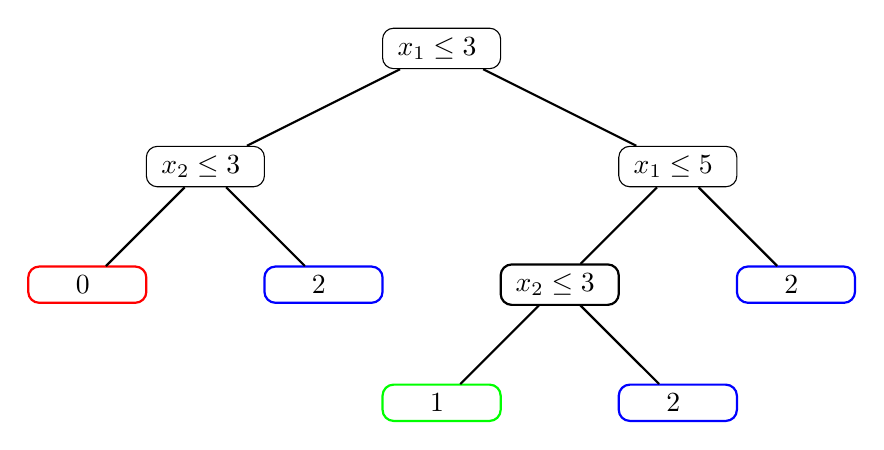
\begin{tikzpicture}[
            level distance=1.5cm,
            edge from parent/.style={draw,thick},
            every node/.style={draw, rounded corners, minimum width=1.5cm, align=center},
            level 1/.style={sibling distance=6cm}, % Separate left and right subtrees
            level 2/.style={sibling distance=3cm}  % Keep children spaced properly
          ]
          
          % Root node
          \node { $x_1 \leq 3$ }
            % Left subtree
            child { node { $x_2 \leq 3$ }
              child { node[draw=red] { 0 } }
              child { node[draw=blue] { 2 } }
            }
            % Right subtree, shifted manually
            child { node { $x_1 \leq 5$ }
              child { node { $x_2 \leq 3$ }
                child { node[draw=green] { 1 } }
                child { node[draw=blue] { 2 } }
              }
              child { node[draw=blue] { 2 } }
            };
          
        \end{tikzpicture}
    \end{center}


\end{example}

